\documentclass{article}

\usepackage{neurips_2026}

\usepackage[utf8]{inputenc}
\usepackage[T1]{fontenc}
\usepackage{hyperref}
\usepackage{url}
\usepackage{booktabs}
\usepackage{tabularx}
\usepackage{amsmath}
\usepackage{amssymb}
\usepackage{graphicx}
\usepackage{subcaption}
\usepackage{microtype}
\usepackage{xcolor}

% percentage-point macro used by generated tables/macros.tex
\newcommand{\pp}{\ensuremath{\,\mathrm{pp}}}

\graphicspath{{figures/}}
\newcommand{\GoldCeilingAcc}{54.7}
\newcommand{\GraphExpansionAcc}{53.8}
\newcommand{\GoldVsGraphP}{0.912}
\newcommand{\GoldVsGraphDelta}{+0.85\pp}
\newcommand{\GoldVsTerseDelta}{+14.53\pp}
\newcommand{\GoldVsTerseP}{0.0005}
\newcommand{\GraphExpansionHard}{42.9}
\newcommand{\GraphRerankingHard}{45.0}
\newcommand{\GraphArbitrationHard}{41.4}
\newcommand{\TailAcc}{46.2}
\newcommand{\CompressAcc}{51.3}
\newcommand{\RAGAcc}{51.7}
\newcommand{\QZeroAcc}{40.2}
\newcommand{\GoldOrigAcc}{41.5}
\newcommand{\GoldOldTwenty}{56.7}
\newcommand{\GoldNewTen}{50.0}
\newcommand{\GraphExpansionOldTwenty}{54.3}
\newcommand{\GraphExpansionNewTen}{52.9}
\newcommand{\GraphArbitrationNewTen}{58.6}
\newcommand{\TotalQuestions}{234}
\newcommand{\QuestionCountOldTwenty}{164}
\newcommand{\QuestionCountNewTen}{70}


\title{Can a Non-Linear Knowledge Graph Make a Small-Model Long-Context\\
Reader Approach the Evidence Ceiling?\\
A Detective-Novel Case Study}

\author{Anonymous Author(s) \\
  Anonymous Affiliation \\
  \texttt{anon@example.com}}

\begin{document}
\maketitle

\begin{abstract}
Large language models read long documents as a \emph{linear} input history: tokens
enter a fixed context window in narrative order, so evidence access depends on
position as much as on relevance. We ask whether a \emph{non-linear} retrieval
system---a knowledge-graph ``mind map'' over the text---lets a small-context model
approach the ceiling of what the evidence itself permits. We freeze one offline
knowledge graph per novel across 30 detective novels and 234 multiple-choice
questions, and evaluate three graph-navigation protocols against a recent-window
baseline, a whole-book compression baseline, a vector-RAG baseline, and a
question-only control, all with a fixed 9B local model under a 16\,K context.
The thirty novels span two frozen graph-build pipelines, so pooled numbers are
descriptive. The de-biased gold oracle---the model shown every official clue
paragraph under a
protocol that removes option-position artifacts---reaches \GoldCeilingAcc\%,
while the question-only control reaches \QZeroAcc\%
(paired \GoldVsTerseDelta{}, $p=\GoldVsTerseP$). Graph-guided evidence expansion
reaches \GraphExpansionAcc\%, statistically indistinguishable from the oracle
($p=\GoldVsGraphP{}$), even though it reads only a handful of graph-selected
paragraphs per question. We further show that an options-first oracle run is an
unreliable
ceiling: it is correct for \textbf{79.4\%} of questions whose answer is option~D
yet only 21.8--40.0\% for A--C, an option-position anchoring artifact that a
de-biasing protocol removes. More broadly, we view graph navigation as an
instance of \emph{non-linear structured memory}---a sparse index a model can hop
across, so that reasoning depends on structure rather than position. We expect
this primitive to matter more as context windows grow toward a million tokens
while documents and long-term memory reach orders of magnitude beyond that.
\end{abstract}

\textbf{Keywords:} long-context reasoning; knowledge-graph retrieval; non-linear
structured memory; small language models; multiple-choice evaluation.

% ============================================================================
\section{Introduction}
\label{sec:intro}

An LLM's context window is a linear history: the model observes the document
token by token and, in a fixed-length window, must decide what to attend to.
For a novel of roughly \mbox{half a million characters} (about $10^5$ tokens)---far
larger than a 16\,K context---the answer to ``why did the killer leave the
canned tea'' may rest in a paragraph near position 0.28 while the model's
effective attention is pinned near the tail \citep{liu2024lost,hsieh2024found}. The
retrieval problem is therefore not ``is the evidence present'' but ``can the
reader navigate to it non-linearly''. Retrieval-augmented generation
\citep{lewis2020rag} mitigates this with a flat similarity index, but it still
treats the document as an ordered byte stream to be sliced.

This paper studies a different primitive: \emph{graph navigation}. A knowledge
graph over the novel---people, locations, clue objects, events, temporal
anchors, and the evidence sentences that mention them, connected by typed
relations---is a non-linear ``mind map''. To answer a question, the model can
hop from the query node to a small set of evidence nodes, staying well within a
small context budget regardless of where the evidence sits in the linear text
(Figure~\ref{fig:schematic}). The central question of this paper is: for a
small, local, long-context model, can such non-linear graph navigation bring the
model close to the \emph{gold ceiling}---the accuracy the model achieves when it
is handed every official clue paragraph? The primitive scales beyond this
testbed: a 1M-token context is still dwarfed by a 100M-token corpus or a
long-term memory store, and the bottleneck there is the same linear access we
study here, not window size.

We construct a clean, frozen benchmark to test this. On 30 detective novels with
234 multiple-choice questions, we fix a 9B local model (16\,K context, chain of
thought disabled) and evaluate (i)~three graph-navigation protocols built from
frozen per-novel graphs, (ii)~three standard retrieval/compression baselines,
(iii)~a question-only control, and (iv)~a \emph{fair gold oracle}: the model
shown all official clue paragraphs under a protocol that removes option-position
artifacts. We measure whether graph navigation approaches the oracle, and we
quantify exactly where the remaining gap comes from.

\begin{figure}[t]
\centering
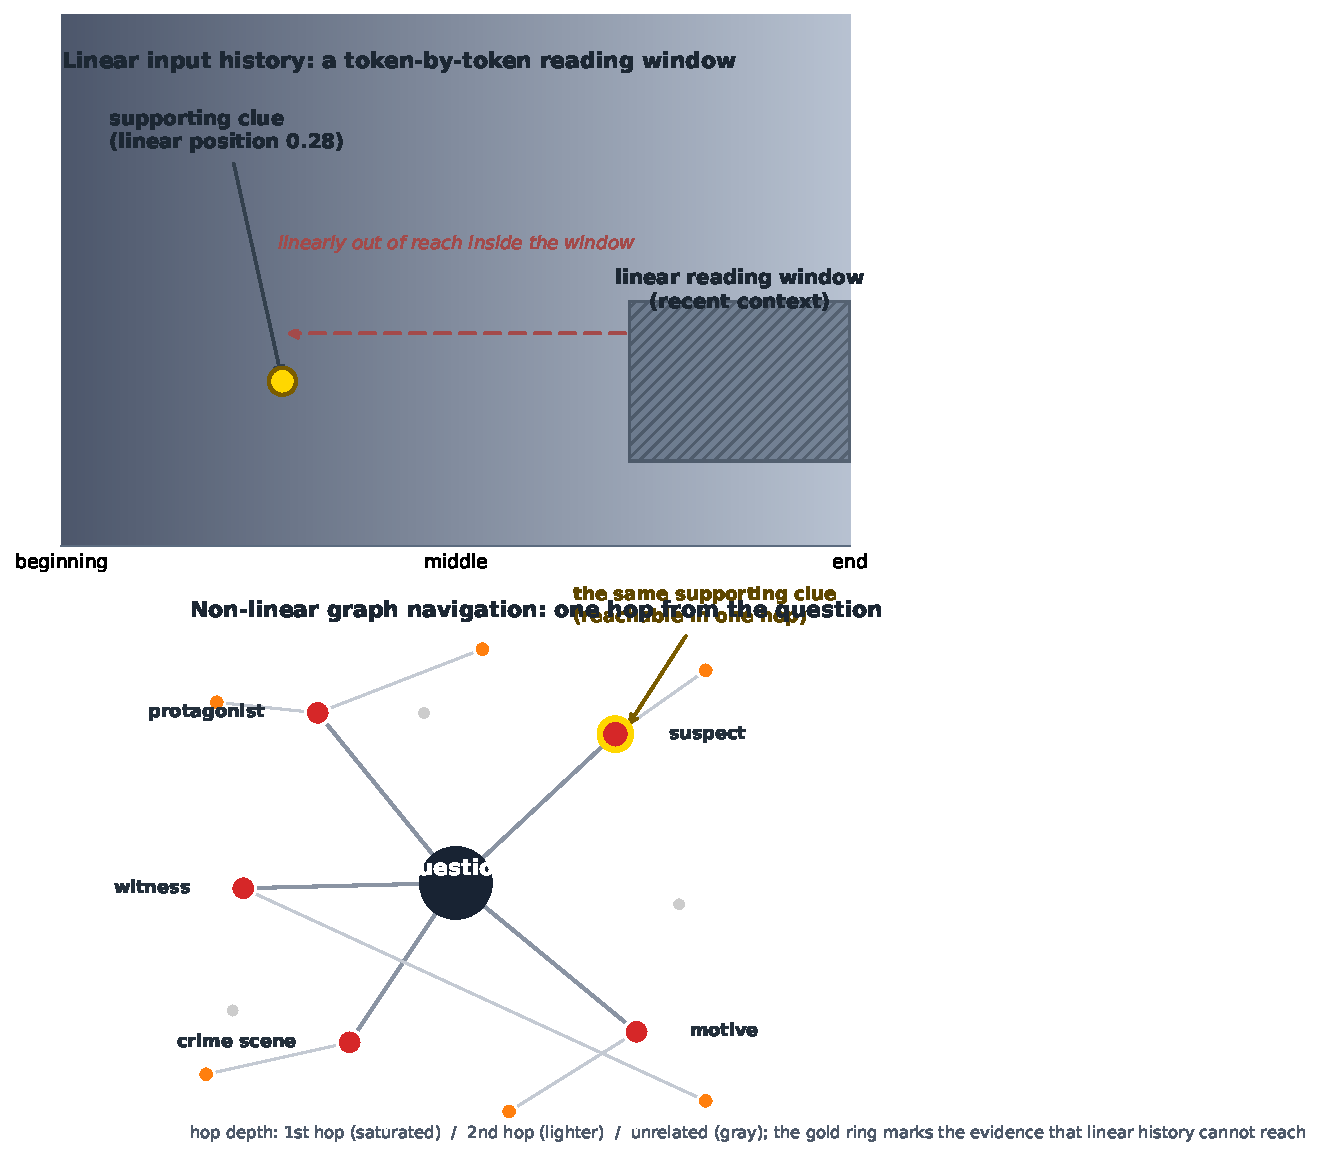
\includegraphics[width=0.92\linewidth]{fig_schematic_linear_vs_graph.pdf}
\caption{
Linear input history vs.\ non-linear graph navigation. \textbf{Top:} the novel is
a $0$--$1$ linear reading ruler; a fixed-size reading window on the tail cannot
see a supporting clue at position 0.28. \textbf{Bottom:} the same clue is one
graph hop from the question node, reachable with a tiny context budget
independently of linear position. Hop depth is encoded by size and color
(1st hop saturated, 2nd hop lighter, unrelated nodes gray) following the
dashboard color convention used throughout our analysis.
}
\label{fig:schematic}
\end{figure}

Our headline results are threefold.

\begin{itemize}
\item \textbf{The de-biased oracle is a real ceiling.} Under a protocol that
shuffles options and presents evidence before options, the gold oracle reaches
\GoldCeilingAcc\% versus \QZeroAcc\% for the question-only control
(\GoldVsTerseDelta{}, paired exact McNemar $p=\GoldVsTerseP{}$); the original
options-first gold run reaches only \GoldOrigAcc\%, equal to the question-only
control (\QZeroAcc\%), because the model anchors on option position.
\item \textbf{Graph navigation approaches the ceiling.} Graph-guided evidence
expansion reaches \GraphExpansionAcc\%, statistically indistinguishable from
the fair gold oracle ($p=\GoldVsGraphP{}$, paired over the same 234 questions),
using only graph-derived evidence. All three graph protocols beat the
recent-window baseline on the harder questions.
\item \textbf{Option-position artifacts must be controlled.} The fair gold
oracle's +14.5\,\pp{} advantage is not visible in the options-first oracle run;
comparing methods to an un-de-biased oracle is meaningless.
\end{itemize}

The paper is organized as follows. Section~\ref{sec:related} situates the work
in long-context and graph-retrieval literature. Section~\ref{sec:method}
describes the three graph-navigation protocols, the baselines, and the de-biased
gold protocol. Section~\ref{sec:setup} details the frozen corpus and statistics.
Section~\ref{sec:results} reports main results, the ceiling analysis, the
option-position artifact, cohort heterogeneity, and hard-question performance.
Section~\ref{sec:discussion} discusses protocol asymmetry and what the results
mean for graph retrieval with small models, followed by limitations
(Section~\ref{sec:limitations}), broader impact (Section~\ref{sec:impact}), and
conclusion (Section~\ref{sec:conclusion}).

% ============================================================================
\section{Related Work}
\label{sec:related}

\textbf{Position bias in long-context models.} LLM performance on long inputs
degrades with the position of relevant content: models favor content at the
beginning and end of long contexts, suffering in the middle
\citep{liu2024lost}, and similar middle-collapse and recency effects have been
reported across model families \citep{hsieh2024found}. Our recent-window
baseline directly measures the recency prior in a clue-dense narrative, and our
de-biased oracle removes an orthogonal artifact: option-position anchoring in
multiple-choice evaluation.

\textbf{Graph-based retrieval.} GraphRAG \citep{edge2024graphrag} constructs a
community hierarchy over an entity graph and answers queries from aggregated
community summaries; HippoRAG \citep{gutierrez2024hipporag} builds a
personalized PageRank-based retrieval over a knowledge graph, and GraphReader
\citep{li2024graphreader} walks a graph with an agentic controller. These
systems optimize for recall on open-ended QA with large frontier models. Our
setting differs in three ways: the graphs are frozen offline artifacts (no
per-query graph construction), the reader is a fixed 9B local model with a
16\,K context, and the outcome is a multiple-choice accuracy against a
de-biased evidence ceiling rather than open-ended generation.

\textbf{Hierarchical and structured memory.} RAPTOR \citep{sarthi2024raptor}
builds a tree of recursively summarized clusters for long-context retrieval, and
LongRAG \citep{zhao2024longrag} retrieves long ``group units'' to push evidence
into the context window. These are linear-to-tree transformations of the text;
our graphs additionally encode typed relations and entity resolution, and we
compare retrieval protocols against an explicit gold-evidence ceiling.

\textbf{Long-context QA datasets.} DetectiveQA \citep{xu2024detectiveqa}
releases detective-novel QA with annotated evidence; our benchmark follows its
question style and uses its clue-position notion for the gold oracle, but fixes
the reader model and freezes the graph artifacts to enable controlled
statistical comparison.

% ============================================================================
\section{Method}
\label{sec:method}

\subsection{Graph representation}
\label{sec:graph}

For each novel we freeze an offline knowledge graph: nodes are typed entities
(\emph{person}, \emph{location}, \emph{clue object}, \emph{event}, \emph{time
anchor}) and \emph{evidence sentences} (paragraphs that mention an entity), and
edges are typed relations (\emph{appears in}, \emph{participates in}, temporal
\emph{before}/\emph{after}, \emph{causes}, \emph{supports}, \emph{contradicts},
\emph{related to}). Graphs are built from the novel text without access to
future questions or gold answers. Each question is grounded in this graph by
matching its entities to nodes, giving a query node from which all graph
protocols start.

\subsection{Graph-navigation protocols}
\label{sec:protocols}

All three protocols answer the same multiple-choice question using only
graph-derived text, with the original option order, and with no access to
baselines or gold.

\textbf{Graph-guided evidence expansion.} The reader expands from the query node
along graph edges to a small set of evidence chunks (order of a handful of
supporting paragraphs), concatenates them with the question and options, and
answers. This is the ``tight'' graph expansion protocol: the context is tiny and
entirely graph-selected.

\textbf{Graph-native chunk reranking.} The reader first builds a candidate pool
of graph-neighbor chunks (order of a few dozen), then re-ranks the pool using
graph-native metadata (hop proximity and entity overlap) to select the top
handful of chunks, and answers from those.

\textbf{Graph-based disagreement arbitration.} The reader runs the first two
protocols as independent graph readers; when their selected answers disagree, a
graph-only referee decides the final answer from the union of their evidence.

\subsection{Baselines and control}
\label{sec:baselines}

We compare against three standard non-graph conditions and one control, all with
the same fixed model and context budget:
\begin{itemize}
\item \textbf{Recent-window baseline.} The reader receives the tail of the novel
  up to the context limit---the natural linear-history baseline.
\item \textbf{Whole-book compression baseline.} The novel is compressed into the
  context window via extractive-compression text, then read.
\item \textbf{Vector RAG baseline.} A flat dense retriever selects chunks by
  question similarity (standard retrieval-augmented generation).
\item \textbf{Question-only control.} The reader sees only the question and
  options---the floor that any evidence-using method must beat.
\end{itemize}

\subsection{The de-biased gold oracle and the option-position artifact}
\label{sec:fairgold}

A gold oracle hands the model every official clue paragraph
\citep{xu2024detectiveqa} and asks it to answer. We found that this oracle, in
its natural \emph{options-first, original-order} form, is useless as a ceiling:
the model is \textbf{79.4\%} accurate when the gold answer is option~D but
21.8--40.0\% for A--C, and selects D on roughly 59\% of all questions. The
oracle is learning where the answer sits, not what it means. We therefore define
the \textbf{fair gold oracle} with a de-biasing protocol: evidence paragraphs are
presented \emph{before} the options, and the option order is shuffled per
question using a permutation derived deterministically from SHA-256 over the
question ID, so the model cannot exploit position and every run is reproducible
from the question IDs alone. We verify the protocol itself is neutral by
re-running the question-only control under the same terse instruction
(``Do not explain. Answer with exactly one line: Answer: [letter]'') and
shuffled options: it achieves the same \QZeroAcc\% pooled as the original
control (per cohort the two diverge---41.5\% vs.\ 37.2\% on the first twenty
and 37.1\% vs.\ 47.1\% on the final ten---so the pooled match is descriptive),
confirming that the +14.5\,\pp{} gain of the oracle is evidence, not instruction
or order.

\subsection{Statistics}
\label{sec:stats-method}

All methods are evaluated on the identical set of 234 questions, so every
comparison is a paired comparison. Primary inference uses exact two-sided
paired McNemar tests on discordant pairs; we report the delta in accuracy
points, wins/losses on discordant pairs, the exact $p$-value, and a
novel-clustered bootstrap 95\% confidence interval (5,000 resamples of whole
novels, so novels are the sampling unit, not questions). Where a family of
graph-vs-baseline contrasts is tested, we apply Holm--Bonferroni correction
across the family of nine contrasts (three graph protocols $\times$ three
baselines). Deltas are reported as first condition minus second condition (e.g.,
oracle minus graph method).

% ============================================================================
\section{Experimental Setup}
\label{sec:setup}

\textbf{Corpus.} 30 detective novels, 234 multiple-choice questions
(164 in the first cohort of 20 novels, 70 in the final cohort of 10). Each
question has four options and an official set of clue paragraphs used for the
gold oracle.

\textbf{Model and context.} A fixed local 9B model with 16\,K context.
Chain-of-thought (CoT) prompting \citep{wei2022chain} elicits step-by-step
reasoning before an answer is produced; we disable CoT for all conditions so
that measured accuracy differences are attributable to the input, not to
decoding strategy, and because our task is short multiple-choice answers where
CoT mostly changes verbosity rather than content. All 2,808 evaluations
(12 conditions $\times$ 234 questions) share this one model: four gold-oracle
variants, three graph protocols, three baselines, and two controls.

\textbf{Frozen graphs and contamination control.} Graphs were built offline and
frozen; answers never enter the graph. The first 20 and final 10 novels use two
different, frozen graph-build pipelines, which we report separately and flag as
a descriptive cohort difference: the earlier pipeline used a 7B extractor and a
sparser relation schema (mean 456 edges per novel), the later pass used the same
9B model as the reader with a denser schema (mean 758 edges per novel), which is
why the two pipelines differ markedly in gold-paragraph recall
(Section~\ref{sec:heterogeneity}). Pooled results across both cohorts are
descriptive and labeled as such.

\textbf{Gold evidence.} For each question, the gold evidence is every official
clue paragraph with a nonnegative clue position; the final-answer paragraph is
excluded. The fair gold oracle concatenates these paragraphs before the
(shuffled) options. The option shuffle is seeded per question ID and applied
identically in all de-biased runs.

\textbf{Metrics.} Micro accuracy on the 234 questions; per-cohort accuracy;
hard-subset accuracy (the 140 questions the question-only control answers
incorrectly, i.e.\ the questions that actually require evidence); per-gold-letter
accuracy; and the paired statistics above.

% ============================================================================
\section{Results}
\label{sec:results}

\subsection{Main results}
\label{sec:mainresults}

Table~\ref{tab:main} and Figure~\ref{fig:main} report pooled accuracy by cohort.
All three graph protocols beat the recent-window baseline and the question-only
control; graph-guided evidence expansion (53.8\%) and graph-based disagreement
arbitration (53.4\%) are the strongest, matching the fair gold oracle
(54.7\%).

\begin{table}[t]
\centering
\caption{
Main results (micro accuracy, \%). ``old20''/``new10'' are the two frozen
cohorts; ``Pooled'' combines them descriptively. ``Hard subset'' is accuracy on the
140 questions the question-only control already fails. The de-biased gold
oracle is the evidence ceiling.
}
\label{tab:main}
\begin{tabular}{lcccc}
\toprule
Method & old20 & new10 & Pooled & Hard subset \\
\midrule
\textbf{Fair gold oracle (gold ceiling)} & 56.7 & 50.0 & \textbf{54.7}\% & 47.1 (66/140) \\
\midrule
Graph-guided evidence expansion & 54.3 & 52.9 & 53.8\% & 42.9 \\
Graph-native chunk reranking & 50.6 & 51.4 & 50.9\% & 45.0 \\
Graph-based disagreement arbitration & 51.2 & 58.6 & 53.4\% & 41.4 \\
\midrule
Recent-window baseline & 48.2 & 41.4 & 46.2\% & 33.6 \\
Whole-book compression baseline & 51.2 & 51.4 & 51.3\% & 37.1 \\
Vector RAG baseline & 52.4 & 50.0 & 51.7\% & 36.4 \\
\midrule
Question-only control & 37.2 & 47.1 & 40.2\% & -- \\
\bottomrule
\end{tabular}
\vspace{2pt}\begin{scriptsize}Pooled values are descriptive: the first 20 and final 10 graphs come from different frozen pipelines. The fair gold oracle is the de-biased upper bound (evidence before options, per-question shuffled options; Section~\ref{sec:fairgold}). The hard subset is the 140 questions the question-only control answers incorrectly (the ones that actually require evidence).\end{scriptsize}

\end{table}

\begin{figure}[t]
\centering
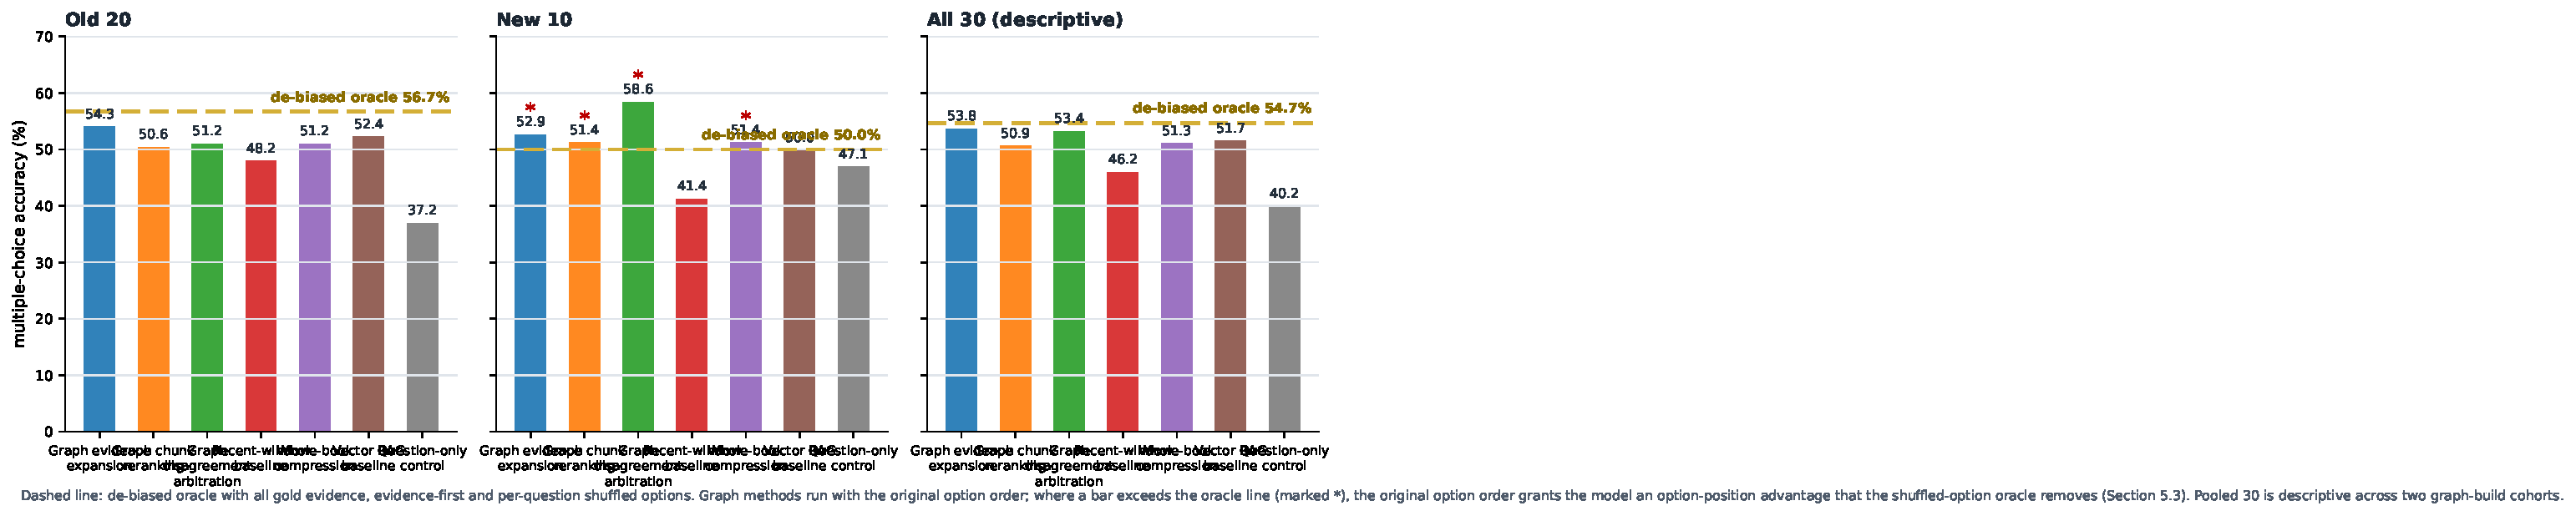
\includegraphics[width=\linewidth]{fig_main_accuracy.pdf}
\caption{
Accuracy by cohort for the seven non-oracle conditions, with the de-biased
oracle as a dashed reference line. Bars marked with ``*'' exceed the oracle line;
these run under the original option order while the oracle shuffles options
(Section~\ref{sec:discussion}), so the position advantage is not exclusive to the
graph conditions---the whole-book compression baseline also crosses the line.
Pooled values are descriptive across the two graph-build cohorts.
}
\label{fig:main}
\end{figure}

\subsection{Closed-source reference points}
\label{sec:closedref}

To situate the local 9B results, Table~\ref{tab:closed} reports a closed-source
frontier model (DeepSeek v4-flash, chain-of-thought disabled) on the same old20
cohort (164 questions). Given the entire novel text it reaches 80.5\%;
restricted to a linear 50{,}000-character tail window it falls to 54.9\%; with
only the question it reaches 41.5\%. Two observations follow. First,
linear-history reading caps even a frontier model at 54.9\% on this cohort, and
only full-novel reading escapes to 80.5\%---the cost of linear access. Second,
the local 9B model reaches 54.3\% through graph navigation alone
(Table~\ref{tab:main}), matching the frontier model's linear tail-reading
accuracy with a small fraction of the context budget; the frontier model's
remaining edge comes from a far larger context window that a 16\,K model cannot
match. This is a descriptive cross-model reference, not a matched comparison:
different models have different intrinsic ceilings, which is precisely why our
main analysis compares each model against a model-specific de-biased oracle.

\begin{table}[t]
\centering
\caption{
External reference points on the old20 cohort (164 questions). ``Linear tail'' is
the final 50{,}000 characters of the novel. The final row repeats the local 9B
graph result for direct comparison.
}
\label{tab:closed}
\begin{tabular}{lcc}
\toprule
Condition & Correct/total & Micro acc. \\
\midrule
Question-only & 68/164 & 41.5\% \\
Linear tail (50\,K chars) & 90/164 & 54.9\% \\
Full novel & 132/164 & 80.5\% \\
\midrule
Graph-guided evidence expansion (local 9B) & 89/164 & 54.3\% \\
\bottomrule
\end{tabular}
\end{table}

\subsection{Graph navigation approaches the gold ceiling}
\label{sec:goldceiling}

The central comparison is the gold oracle against the question-only control and
the graph protocols (Table~\ref{tab:paired}, Figure~\ref{fig:pairwise}).
The fair gold oracle exceeds the question-only control by
\GoldVsTerseDelta{} (63 wins vs.\ 29 losses on discordant pairs,
$p=\GoldVsTerseP{}$, 95\% CI $[6.9, 23.4]$\,\pp). This is the evidence effect: the
same 9B model, given all official clues under a position-neutral protocol,
moves 14.5 accuracy points. Graph-guided evidence expansion, given only a
handful of graph-derived paragraphs, reaches \GraphExpansionAcc\%, and the
paired contrast against the oracle is $+0.85$\,\pp{} ($p=0.912$; deltas are
reported as first condition minus second, so $+0.85$ favors the oracle): the
graph reader is statistically indistinguishable from a reader handed the
complete gold evidence. Graph-based disagreement arbitration is likewise
indistinguishable ($+1.28$\,\pp, $p=0.832$, also favoring the oracle).

\begin{table}[t]
\centering
\caption{
Paired contrasts over the same 234 questions (exact two-sided McNemar; W/L =
wins/losses on discordant pairs; 95\% CI is the novel-clustered bootstrap).
The top block shows the gold-oracle analysis; the bottom block shows graph
methods against the recent-window baseline with Holm-corrected $p$.
}
\label{tab:paired}
% L = ragged-right wrapping label column; R = wrapping CI column.
\newcolumntype{L}{>{\raggedright\arraybackslash}X}
\newcolumntype{R}{>{\raggedright\arraybackslash}p{2.2cm}}
\small
\begin{tabularx}{\linewidth}{L rrrrR}
\toprule
Paired contrast & $\Delta$ & W/L & exact $p$ & Holm $p$ & bootstrap 95\% CI \\
\midrule
Fair gold vs. question-only (terse) & +14.53pp & 63/29 & \textbf{0.0005} & -- & [6.9, 23.4] \\
Fair gold vs. graph-guided expansion & +0.85pp & 42/40 & 0.912 & -- & [-5.9, 8.0] \\
Fair gold vs. graph arbitration & +1.28pp & 46/43 & 0.832 & -- & [-6.6, 9.7] \\
Options-first gold vs. question-only (artifact) & +1.28pp & 43/40 & 0.826 & -- & [-4.9, 7.8] \\
\midrule
Graph-guided expansion vs. recent-window (pooled) & +7.69pp & 47/29 & 0.050 & 0.454 & [2.0, 13.9] \\
Graph arbitration vs. recent-window (new10) & +17.14pp & 15/3 & 0.008 & 0.068 & [5.4, 31.9] \\
\bottomrule
\end{tabularx}
\vspace{2pt}\begin{scriptsize}Exact two-sided paired McNemar over the same 234 questions; \textit{W/L} = wins/losses on discordant pairs. Bootstrap deltas are novel-clustered (5,000 resamples of whole novels).\end{scriptsize}

\end{table}

\begin{figure}[t]
\centering
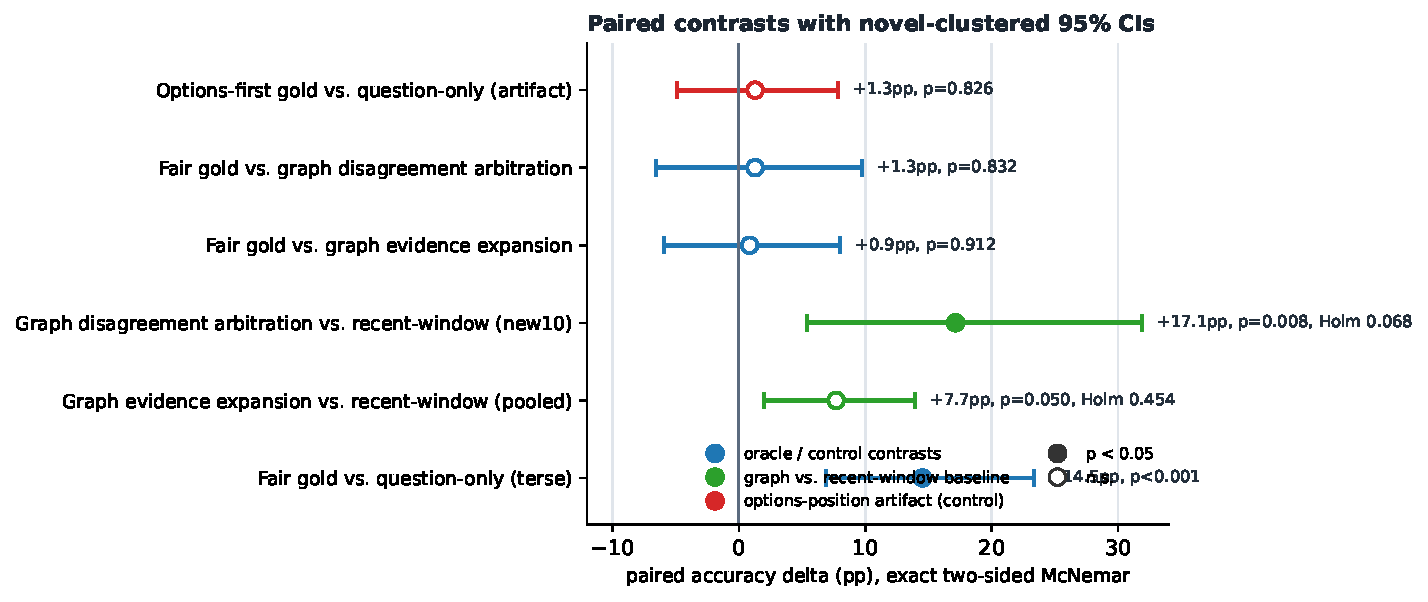
\includegraphics[width=\linewidth]{fig_pairwise.pdf}
\caption{
Forest plot of the key paired contrasts. Filled markers are significant at
$p<0.05$; error bars are novel-clustered bootstrap 95\% CIs. The headline
evidence effect (fair gold vs.\ question-only) is +14.5\,\pp, while the graph
methods are indistinguishable from the fair gold oracle.
}
\label{fig:pairwise}
\end{figure}

\subsection{Option-position anchoring is a methodological artifact}
\label{sec:danchor}

Figure~\ref{fig:danchor} and Table~\ref{tab:danchor} (Appendix) document why an
oracle must be de-biased. The options-first gold oracle---all evidence, options
first, original order---scores \GoldOrigAcc\%, statistically indistinguishable
from the question-only control (\QZeroAcc\%), yet this is not a ``no evidence
helps'' result: the oracle is 79.4\% accurate when the gold answer is D (the
gold letter is D on 65 of the 234 questions) but 21.8--40.0\% for A--C, at or
below the control's per-letter levels. The 9B model anchors on the position of
the options. Shuffling options and moving evidence first removes the artifact:
per-letter accuracy flattens (A 55.2\%, B 47.2\%, C 53.4\%, D 61.5\% for the
fair oracle) and the selected-letter distribution matches the content-implied
gold-letter distribution.

\begin{figure}[t]
\centering
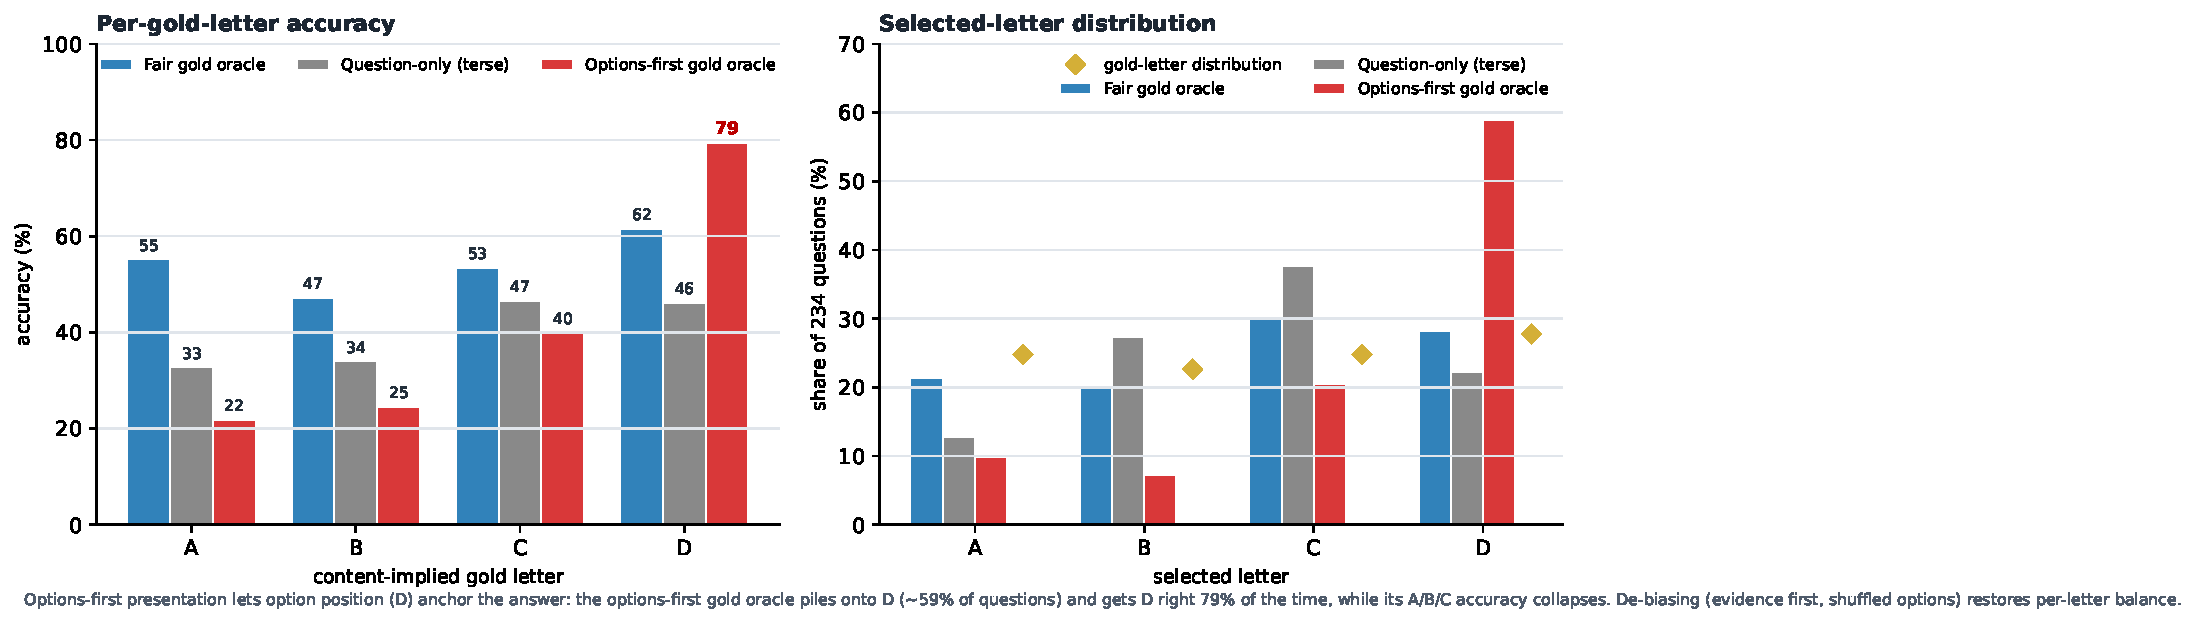
\includegraphics[width=\linewidth]{fig_d_anchoring.pdf}
\caption{
\textbf{Left:} per-gold-letter accuracy. The options-first oracle is
21.8--40.0\% for A--C (at or below the control's per-letter levels) but 79.4\%
for D (highlighted), the anchoring signature.
\textbf{Right:} selected-letter distribution (share of questions); the
options-first oracle piles onto D (~59\%), while the de-biased oracle tracks the
content-implied gold-letter distribution.
}
\label{fig:danchor}
\end{figure}

\subsection{Cohort heterogeneity}
\label{sec:heterogeneity}

The two frozen cohorts behave very differently, which drives the pooled numbers.
In the old20 cohort the gold evidence sits overwhelmingly in the graph's
2-core---the gold-overlap rate is 53.7\% versus 18.2\% for other nodes
(enrichment 2.95, odds ratio 5.21), and graph retrieval reaches only 16.3\% of
gold paragraphs. In the new10 cohort the graph build is far more complete:
73.2\% of gold paragraphs are retrieved, the enrichment is 1.61 (odds ratio
2.32), and the best graph protocol reaches \GraphArbitrationNewTen\%
(versus \GoldNewTen\% for the de-biased oracle under its more conservative
protocol). The two cohorts therefore bound the failure and success modes of the
graph pipeline.

\subsection{Hard-question performance}
\label{sec:q0hard}

The 140 questions the question-only control gets wrong are the ones that
actually require evidence. On this subset the fair gold oracle reaches 47.1\%
(66/140); graph-native chunk reranking reaches 45.0\%, graph-guided evidence
expansion 42.9\%, and graph-based disagreement arbitration 41.4\%. Every graph
protocol beats the recent-window baseline (33.6\%) and the compression (37.1\%)
and RAG (36.4\%) baselines. The gap to the oracle on hard questions is where the
graph pipeline loses evidence, not where the reader fails to reason.

\subsection{Summary of paired statistics}
\label{sec:stats}

Across the family of nine graph-vs-baseline contrasts, graph-guided evidence
expansion vs.\ recent-window is the strongest pooled signal
(+7.69\,\pp, $p=0.050$, Holm-corrected $p=0.454$); on the new10 cohort,
graph-based disagreement arbitration vs.\ recent-window is +17.14\,\pp
(15 wins vs.\ 3 losses, $p=0.008$, Holm-corrected $p=0.068$). The Holm
correction is conservative for a 9-comparison family; we report exact and
corrected values throughout.

% ============================================================================
\section{Discussion}
\label{sec:discussion}

\textbf{Graph navigation converts position into topology.} The mechanism behind
the headline result is visible in Figure~\ref{fig:schematic}: for a small model
with a fixed 16\,K context, the question is not whether the clue exists in the
book but whether the reader can reach it. A graph hop costs the same budget
whether the target sits at linear position 0.05 or 0.95. Graph-guided evidence
expansion uses a few hundred tokens of graph-selected evidence and matches a
reader given the full official clue set---the graph is, in effect, a
non-linear index that lets the model spend its small context where the answer
is.

\textbf{Protocol asymmetry favors the graph methods.} The fair gold oracle
shuffles options and presents evidence first; the graph protocols run the
original option order. Shuffling options is harder for a position-sensitive 9B
model, so the oracle's 54.7\% is a conservative ceiling. This is why, on the
new10 cohort, graph methods can exceed the de-biased oracle line
(Figure~\ref{fig:main}): under the original option order the same evidence is
worth more to this model. The asymmetry means our ``indistinguishable from the
ceiling'' claim is, if anything, conservative.

\textbf{Where the graph loses.} The gap between graph methods and the oracle is
almost entirely retrieval-side: on the hard questions the graph protocols reach
41--45\% versus 47.1\% for the oracle, and cohort heterogeneity shows the gap
is largest precisely where graph recall is lowest (old20: 16.3\% gold recall).
Graph-based disagreement arbitration partially recovers lost evidence by
running two readers and arbitrating their disagreement, which is why it is the
best protocol on the stronger new10 cohort (58.6\%).

\textbf{Small models are the right testbed.} A frontier model with a large
context and strong instruction following may ``search'' linearly within its
window; a 9B model with 16\,K context cannot. Our results show the graph
primitive matters most for exactly this regime---the regime of local,
on-device, cost-sensitive deployment.

\textbf{Toward non-linear structured memory.} Our graphs instantiate a general
primitive: a structured memory a reader queries by navigation rather than by
linear scan. Attention over a long history is expensive and position-biased; a
sparse index trades a small retrieval cost for freedom from position. The
direction scales: a model with a 1M-token context asked to reason over a
100M-token corpus or long-term memory store faces the same problem a 16\,K model
faces with a half-million-character novel---the evidence is somewhere in the
history, but the reader cannot afford to see all of it. If navigation is what
let the small model approach its evidence ceiling here, the same non-linear
index may be what lets much larger models approach their ceilings on histories
two orders of magnitude beyond their windows.

% ============================================================================
\section{Limitations}
\label{sec:limitations}

\textbf{Heterogeneous graph pipelines.} The two cohorts use different frozen
graph builds; pooled numbers are descriptive, and per-cohort results must be
read separately. A single, uniform graph pipeline is needed to make the pooled
claim strong.

\textbf{Exploratory development on the corpus.} The graph protocols were
developed on these 30 novels; the fixed 9B model and frozen graphs reduce but do
not eliminate selection bias. The gold and baseline conditions are independent
of the graph development, which protects the ceiling comparison.

\textbf{Single model.} All conclusions are for one 9B checkpoint. The
de-biasing protocol and the ceiling comparison should transfer, but the exact
magnitudes are model-specific.

\textbf{Lexical gold matching.} Gold evidence is matched to paragraphs by the
dataset's clue positions; the gold oracle sees the official clue set, not
necessarily every sentence that could help.

\textbf{No attention-level causality.} We show accuracy differences, not a
mechanism; we do not trace attention to graph-selected versus linear evidence.

\textbf{Contamination nuance.} Graphs are built from the full novel, so a graph
node may touch the answer region; the graph protocols can surface content
beyond the official clue set. This makes the oracle comparison conservative
(the oracle is restricted to official clues) but means the graph's ceiling
itself is not bounded by the official clue set.

% ============================================================================
\section{Broader Impact}
\label{sec:impact}

This is low-risk research on synthetic-style QA over public-domain detective
fiction; no user data, no generation of harmful content. The main transferable
finding is methodological: \emph{multiple-choice evaluation of small models is
sensitive to option order}, and gold/oracle runs that do not shuffle options
can produce systematically misleading ceilings (79.4\% on D, 21.8--40.0\%
elsewhere). We recommend that MCQ evaluations of long-context systems shuffle
options with a fixed seed and, for evidence ceiling estimation, present
evidence before options. The graph-retrieval primitive itself has
straightforward applications in document QA where context budgets are tight.

% ============================================================================
\section{Conclusion}
\label{sec:conclusion}

We showed that a non-linear knowledge-graph retrieval system lets a small,
fixed-context model approach the evidence ceiling on long detective-novel
reasoning. Under a de-biased protocol, the gold oracle is a genuine ceiling
(+14.5\,\pp{} over the question-only control), and graph-guided evidence
expansion is statistically indistinguishable from it ($p=0.912$), while three
different graph protocols all outperform linear-history baselines on the
questions that require evidence. We also documented an option-position
anchoring artifact that makes naive gold oracles unreliable. For small models
with tight context budgets, graph navigation is a cheap, effective substitute
for linear search. Looking forward, we treat the graph as the simplest form of
non-linear structured memory: a sparse index that lets a model spend its
attention where the answer is, independent of position. The bottleneck of
linear access does not shrink as windows grow, so we expect this primitive to
matter more as models move to million-token contexts over corpora and memories
of a hundred million tokens or more.

% ============================================================================
\bibliographystyle{plainnat}
\bibliography{references}

% ============================================================================
\appendix
\section{Full cohort results}
\label{app:full}
\begin{tabular}{lcc}
\toprule
Method & correct/total & micro acc. (old20) \\
\midrule
Fair gold oracle (gold ceiling) & 93/164 & 56.7\% \\
Gold oracle (evidence-first, original order) & 97/164 & 59.1\% \\
Gold oracle (options-first, shuffled) & 88/164 & 53.7\% \\
Options-first gold oracle & 63/164 & 38.4\% \\
Graph-guided evidence expansion & 89/164 & 54.3\% \\
Graph-native chunk reranking & 83/164 & 50.6\% \\
Graph-based disagreement arbitration & 84/164 & 51.2\% \\
Recent-window baseline & 79/164 & 48.2\% \\
Whole-book compression baseline & 84/164 & 51.2\% \\
Vector RAG baseline & 86/164 & 52.4\% \\
Question-only control (terse) & 68/164 & 41.5\% \\
Question-only control & 61/164 & 37.2\% \\
\bottomrule
\end{tabular}

\begin{tabular}{lcc}
\toprule
Method & correct/total & micro acc. (new10) \\
\midrule
Fair gold oracle (gold ceiling) & 35/70 & 50.0\% \\
Gold oracle (evidence-first, original order) & 38/70 & 54.3\% \\
Gold oracle (options-first, shuffled) & 35/70 & 50.0\% \\
Options-first gold oracle & 34/70 & 48.6\% \\
Graph-guided evidence expansion & 37/70 & 52.9\% \\
Graph-native chunk reranking & 36/70 & 51.4\% \\
Graph-based disagreement arbitration & 41/70 & 58.6\% \\
Recent-window baseline & 29/70 & 41.4\% \\
Whole-book compression baseline & 36/70 & 51.4\% \\
Vector RAG baseline & 35/70 & 50.0\% \\
Question-only control (terse) & 26/70 & 37.1\% \\
Question-only control & 33/70 & 47.1\% \\
\bottomrule
\end{tabular}

\begin{tabular}{lcc}
\toprule
Method & correct/total & micro acc. (pooled) \\
\midrule
Fair gold oracle (gold ceiling) & 128/234 & 54.7\% \\
Gold oracle (evidence-first, original order) & 135/234 & 57.7\% \\
Gold oracle (options-first, shuffled) & 123/234 & 52.6\% \\
Options-first gold oracle & 97/234 & 41.5\% \\
Graph-guided evidence expansion & 126/234 & 53.8\% \\
Graph-native chunk reranking & 119/234 & 50.9\% \\
Graph-based disagreement arbitration & 125/234 & 53.4\% \\
Recent-window baseline & 108/234 & 46.2\% \\
Whole-book compression baseline & 120/234 & 51.3\% \\
Vector RAG baseline & 121/234 & 51.7\% \\
Question-only control (terse) & 94/234 & 40.2\% \\
Question-only control & 94/234 & 40.2\% \\
\bottomrule
\end{tabular}

\begin{tabular}{lc}
\toprule
Method & preservation on control-correct (pooled) \\
\midrule
Graph-guided evidence expansion & 70.2\% \\
Graph-native chunk reranking & 59.6\% \\
Graph-based disagreement arbitration & 71.3\% \\
Recent-window baseline & 64.9\% \\
Whole-book compression baseline & 72.3\% \\
Vector RAG baseline & 74.5\% \\
Options-first gold oracle & 57.4\% \\
\bottomrule
\end{tabular}


\section{De-biased gold analysis (per-letter and distribution)}
\label{sec:danchor-app}
\begin{table}[t]
\centering
\caption{
Per-gold-letter accuracy (left) and selected-letter distribution (right) for the
de-biased and control runs, with the content-implied gold-letter distribution
for reference. The options-first oracle's D spike is an anchoring artifact.
}
\label{tab:danchor}
\begin{subtable}{\linewidth}
\centering
\caption{Per-gold-letter accuracy}
\small
\begin{tabular}{lcccc}
\toprule
Run & A & B & C & D \\
\midrule
Fair gold oracle & 55.2\% & 47.2\% & 53.4\% & 61.5\% \\
Question-only (terse) & 32.8\% & 34.0\% & 46.6\% & 46.2\% \\
Options-first gold oracle & 21.8\% & 24.5\% & 40.0\% & \textbf{79.4}\% \\
\bottomrule
\end{tabular}
\end{subtable}
\vspace{6pt}
\begin{subtable}{\linewidth}
\centering
\caption{Selected-letter distribution}
\small
\begin{tabular}{lcccc}
\toprule
Run & A & B & C & D \\
\midrule
Fair gold oracle & 50 (21.4\%$^{\dagger}$) & 47 (20.1\%$^{\dagger}$) & 71 (30.3\%$^{\dagger}$) & 66 (28.2\%$^{\dagger}$) \\
Question-only (terse) & 30 (12.8\%$^{\dagger}$) & 64 (27.4\%$^{\dagger}$) & 88 (37.6\%$^{\dagger}$) & 52 (22.2\%$^{\dagger}$) \\
Options-first gold oracle & 23 (9.8\%$^{\dagger}$) & 17 (7.3\%$^{\dagger}$) & 48 (20.5\%$^{\dagger}$) & 138 (59.0\%$^{\dagger}$) \\
Gold-letter distribution & 58 (24.8\%$^{\dagger}$) & 53 (22.6\%$^{\dagger}$) & 58 (24.8\%$^{\dagger}$) & 65 (27.8\%$^{\dagger}$) \\
\bottomrule
\end{tabular}
\end{subtable}
\vspace{2pt}\begin{scriptsize}
 $^{\dagger}$Column shares are percent of the 234 questions. The options-first gold oracle piles onto D (138/234 = 59\% of questions) regardless of content, while the de-biased fair gold oracle matches the content-implied gold distribution. The options-first oracle refused to select a letter on 8 questions (its row sums to 226).
\end{scriptsize}

\end{table}

\section{Graph structure analysis}
\label{app:graph}
\begin{figure}[t]
\centering
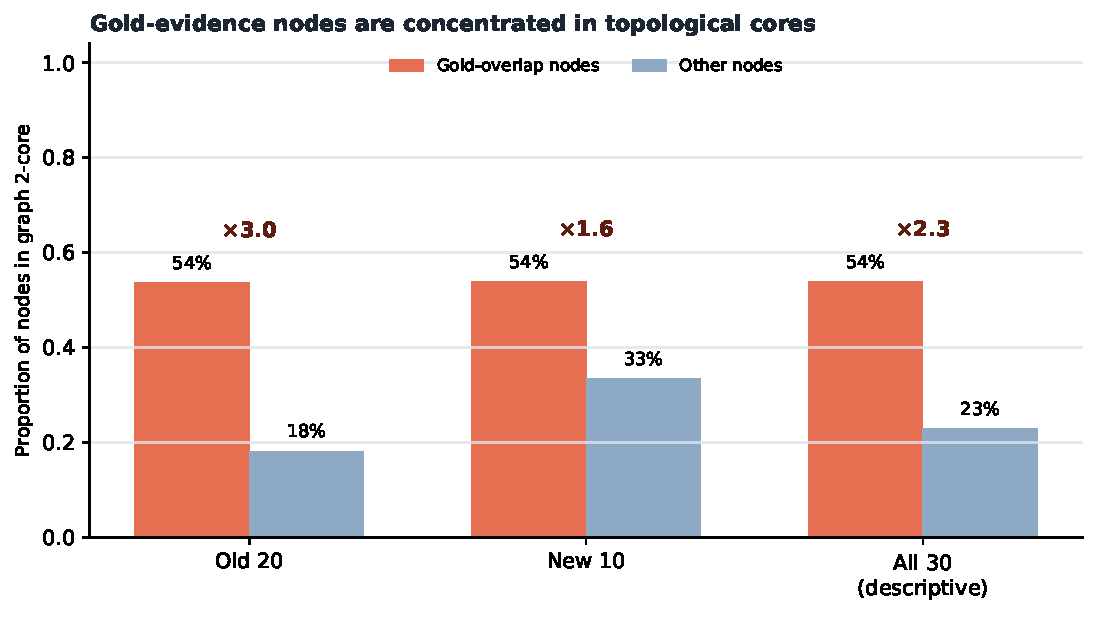
\includegraphics[width=\linewidth]{fig_core_enrichment.pdf}
\caption{
Gold-overlap nodes are concentrated in the topological 2-core of the graph.
Rates are micro over all graph nodes per cohort; ``$\times$'' labels are the
gold/other rate ratio (enrichment).
}
\label{fig:coreenrichment}
\end{figure}

\begin{figure}[t]
\centering
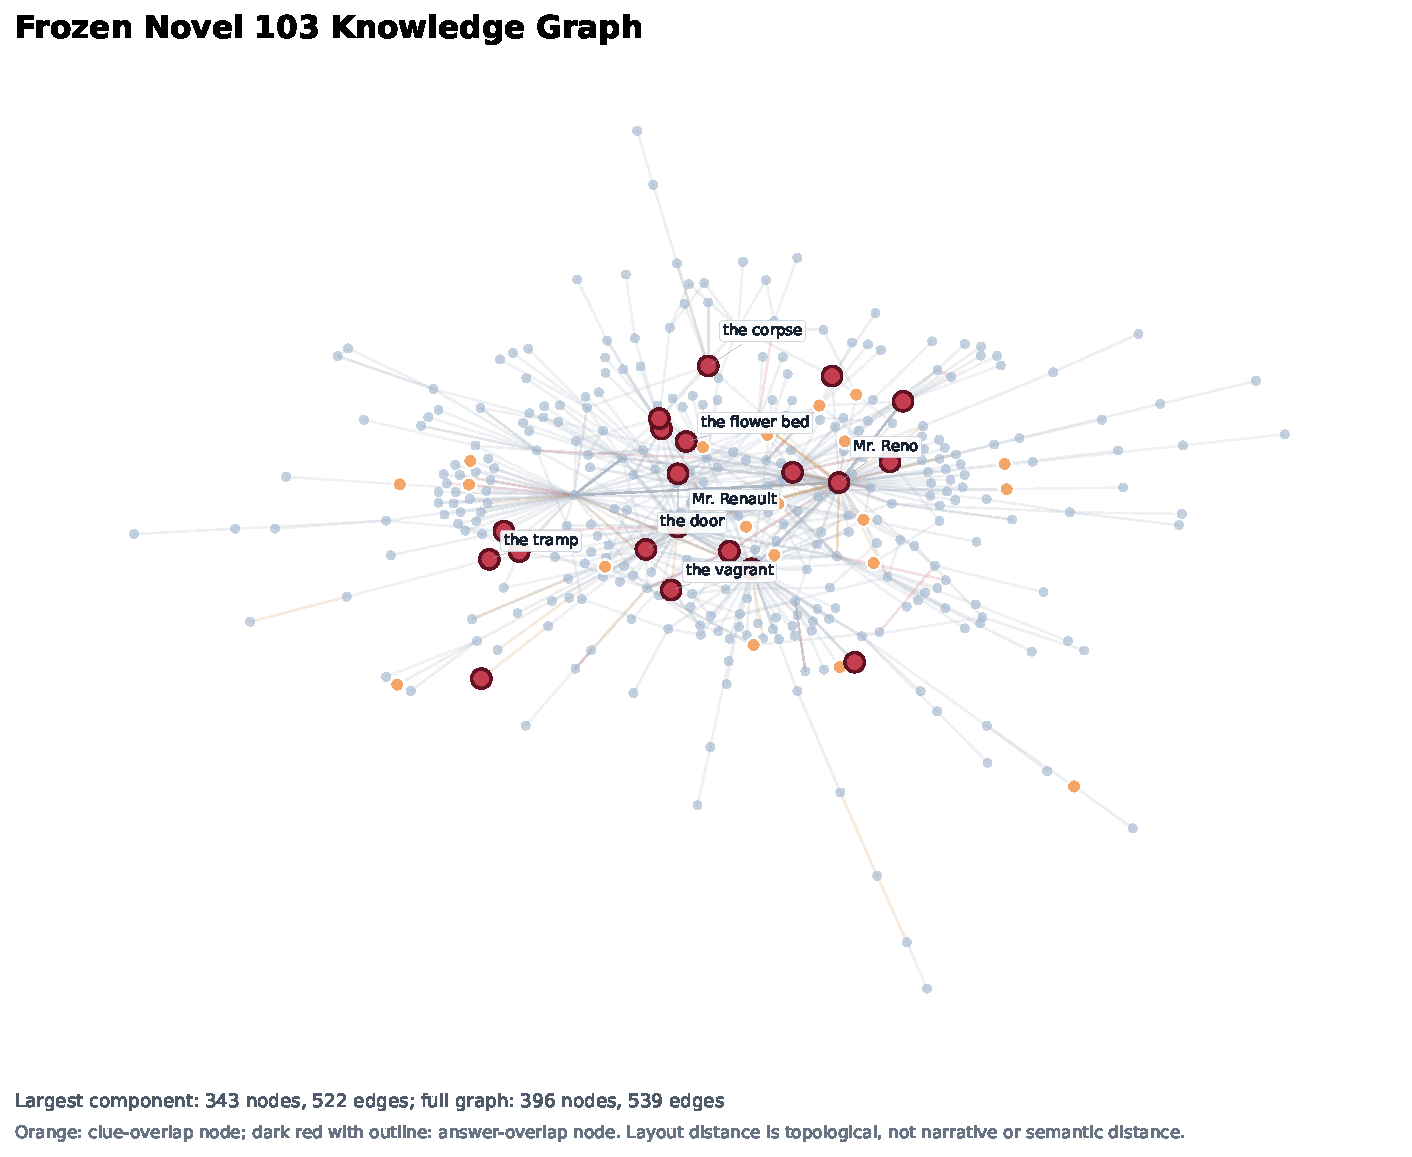
\includegraphics[width=0.72\linewidth]{fig_force_novel103.pdf}
\caption{
Frozen force-layout graph for one novel (n nodes and m edges as annotated).
Orange nodes overlap gold evidence; red nodes overlap the answer. The dashed
circle marks the topological core. Force-layout distance is topological, not
narrative or semantic.
}
\label{fig:force}
\end{figure}

% ============================================================================
\newpage
\input{checklist}

\end{document}
